\documentclass{article}
\usepackage{../verslagstyle}



\begin{document}
	\title{Labo 4}
	\author{Bert De Saffel}
	\date{05 maart 2019}
	\maketitle
	
	\section{Gebruikte functies}
	\begin{itemize}
		 \item \textbf{warpAffine(src, M, dsize[, ...]) $\rightarrow$ dst}
		 
		 Deze functie voert een eenvoudige transformatie uit met de gegeven $2\times 3$ matrix $M$, waarbij $m_x$ en $m_y$ de shear factor voor respectievelijk de horizontale en de verticale richting is. Er kan ook een horizontale of verticale translatie gedefinieerd worden met respectievelijk $o_x$ en $o_y$.
		 
		 $$M = \begin{bmatrix}
		 1 & m_x & o_x \\
		 m_y & 1 & o_y
		 \end{bmatrix}$$
		 
		 Elke pixel in de resultaatimage wordt dan als volgt gemapt:
		 
		 $$dst(x, y) = src(M_{11}x + M_{12}y + M_{13}, M_{21}x + M_{22}y + M_{23})$$
		 
		 Het labo vraagt om horizontale shearing toe te passen, zodat zeker $m_y = 0$ moet zijn, met als gevolg dat $o_y = 0$ mag blijven. De $y$-waarde van elke pixel blijft dus gelijk:
		 
		 $$dst(x, y) = src(M_{11}x + M_{12}y + M_{13}, y) $$
		 
		 Elke $x$-waarde moet wel naar rechts verschoven worden om de schaduw recht te krijgen. Een positieve waarde voor $m_x$ zou, zal altijd een grotere $x$-waarde opleveren dan de originele figuur, zodat de shearing eruit zal zien zoals op figuur \ref{fig:shear_wrong}.
		\begin{figure}[!htb]
		 	\begin{minipage}{0.48\textwidth}
		 	\centering
			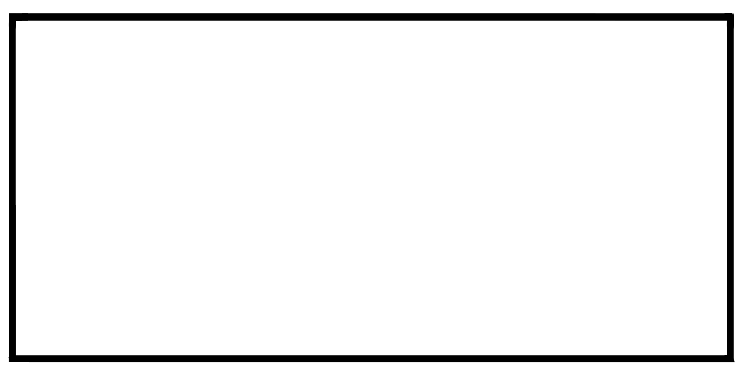
\includegraphics[width=0.9\linewidth]{shear_wrong_original}
			\caption{Originele image.}
			\label{fig:shear_wrong_original}
		 	\end{minipage}\hfill
		 	\begin{minipage}{0.48\textwidth}
		 	\centering
			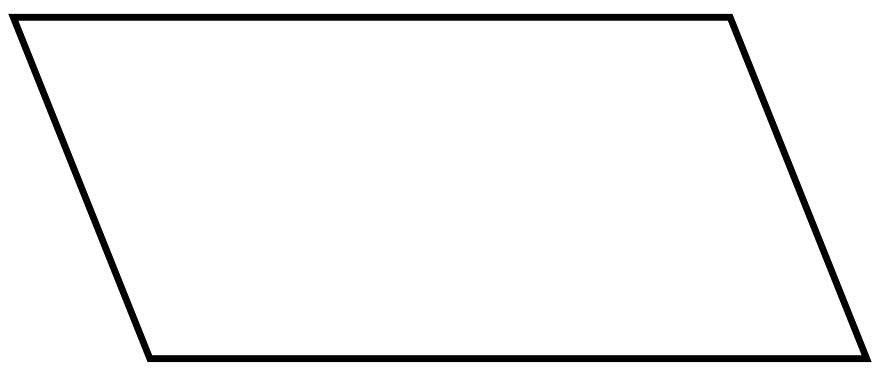
\includegraphics[width=0.9\linewidth]{shear_wrong}
			\caption{Shearing voor een positieve $m_x$ factor.}
			\label{fig:shear_wrong}
		 	\end{minipage}
		 \end{figure}
		 Dit is natuurlijk de foute richting want de schaduw zal nog meer vervormd zijn. Er wordt dus een negatieve waarde voor $m_x$ gekozen. De waarde $m_x = -0.2$ met een horizontale translatie $o_x = 50$ lijkt goed te werken.
		 
		 $$dst(x, y) = src(x - 0,2y + 50, y) $$
		 
		 
		 
		 
		 \item \textbf{setMouseCallback(windowName, onMouse, param=None) $\rightarrow$ None}
		 
		 Deze functie zal een mouse handler initialiseren voor de opgegeven window. OpenCV heeft de mouse handler zo geïmplementeerd dat bij elke beweging van de muis over de opgegeven window een callbackfunctie \textit{onMouse} wordt opgeroepen. Deze callbackfunctie mag eender welke naam hebben, maar het moet wel refereren naar een functie met volgende signatuur (in Python):
		 
		 $$\texttt{onMouse(event, x, y, flags, userdata)} \rightarrow \texttt{None}$$
		 
		 De \textit{event} parameter is een constante die refereert naar het soort event. Voorbeelden van events zijn \texttt{EVENT\_LBUTTONDOWN} voor wanneer de linkermuisknop ingedrukt wordt, \texttt{EVENT\_RBUTTONUP} voor wanneer de rechtermuisknop terug losgelaten wordt, enz. De $x$ en $y$ parameters zijn de coördinaten waar de muis zich bevindt op het moment dat de callbackfunctie opgeroepen wordt. De \textit{flags} parameter geeft nog extra, maar beperkte, informatie zoals bijvoorbeeld of de CTRL toets ingedrukt was of niet. De \textit{userdata} parameter laat toe om optioneel eigen data mee te geven aan de functie.
		 
		 

		 \item \textbf{getPerspectiveTransform(src, dst) $\rightarrow$ retval}
		 
		 Deze functie berekent de $3\times 3$ perspectieve transformatiematrix voor een verzameling van vier coördinaten $src$, en mapt deze op vier andere coördinaten $dst$. Het resultaat van deze functie is een $3 \times 3$ matrix $M$ zodat
		 
		 $$\begin{bmatrix}
		 t_ix_i' \\
		 t_iy_i' \\
		 t_i
		 \end{bmatrix} = M \cdot \begin{bmatrix}
		 x_i \\
		 y_i \\
		 1
		 \end{bmatrix} $$
		 
		 met
		 
		 $$dst(i) = (x_i', y_i'), src(i) = (x_i, y_i), i = 0, 1, 2, 3$$
		 
		 Deze functie doet dus niets anders dan de matrix geven om vier punten punt met coördinaat $(x_i, y_i)$ te mappen op vier andere punten met coördinaat $(x_i', y_i')$ voor $i = 0, 1, 2, 3$. Deze matrix kan dan gebruikt worden door de functie \textit{warpPerspective} om een werkelijke perspectieve transformatie door te voeren.
		 
		 De $src$ coördinaten worden in dit labo aan de gebruiker gevraagd. De parameter $dst$ is hardgecodeerd en stelt de coördinaten van de hoekpunten van een rechthoek voor: 
		 
		 $$(100, 200), (200, 200), (200, 500), (100, 500)$$
		 
		 Het is dan ook een vereiste om de hoekpunten zo aan te klikken zoals op figuur \ref{Fig:ex8_1}.
		 
		 \item \textbf{warpPerspective(src, M, dsize[, ...]) $\rightarrow$ dst}
		 
		Deze functie zal de $src$ image omvormen met een $3 \times 3$ matrix $M$ zodat
		
		$$dst(x, y) = src\bigg(\frac{M_{11}x + M_{12}y + M_{13}}{M_{31}x + M_{32}y + M_{33}}, \frac{M_{21}x + M_{22}y + M_{23}}{M_{31}x + M_{32}y + M_{33}}\bigg)$$
		 
		 De matrix $M$ kan gegenereerd worden met de functie \textit{getPerspectiveTransform}.
		
		
	\end{itemize}
\newpage
	\section{Invoer en uitvoer}
	
	\subsection*{Opgave 7}
	\begin{figure}[!htb]
		\begin{minipage}{0.4\textwidth}
			\centering
			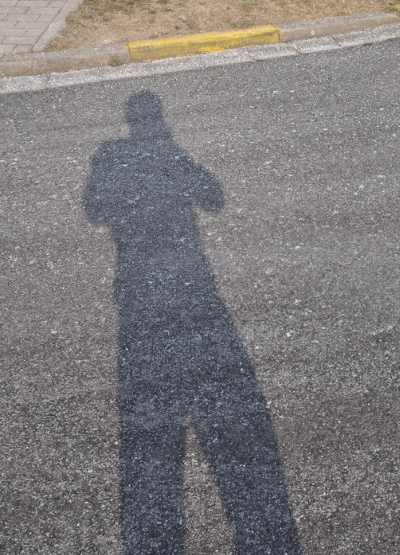
\includegraphics[width=0.9\linewidth]{shadow}
			\caption{De originele figuur.}
			\label{Fig:ex7_1}
		\end{minipage}\hfill
		\begin{minipage}{0.4\textwidth}
			\centering
			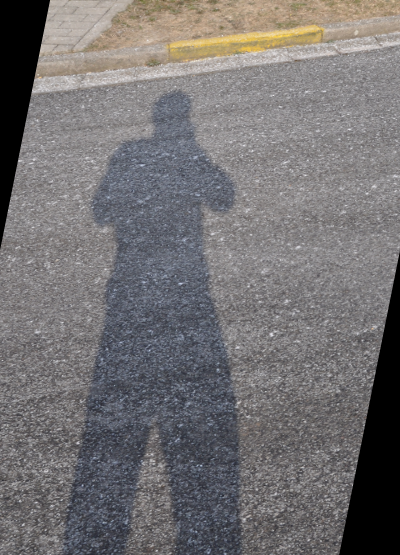
\includegraphics[width=0.9\linewidth]{shadowEX8}
			\caption{Na de horizontale shearing.}
			\label{Fig:ex7_2}
		\end{minipage}\hfill
	\end{figure}
	

	\subsection*{Opgave 8}
	\begin{figure}[!htb]
		\begin{minipage}{0.4\textwidth}
			\centering
			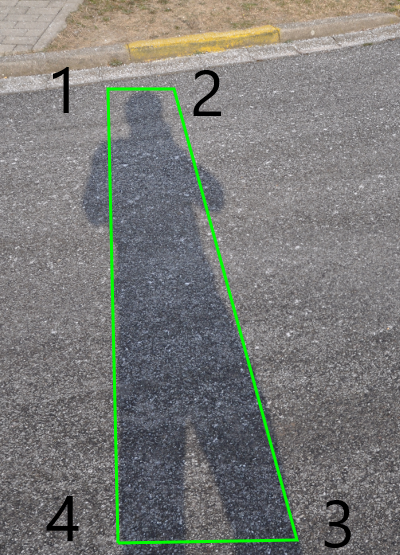
\includegraphics[width=0.9\linewidth]{shadow_box_numbered}
			\caption{De originele figuur. De getallen bij elke hoek stellen de volgorde voor waarin ze aangeklikt moeten worden.}
			\label{Fig:ex8_1}
		\end{minipage}\hfill
		\begin{minipage}{0.4\textwidth}
			\centering
			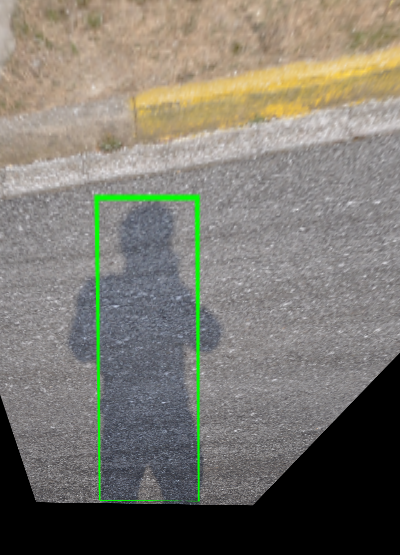
\includegraphics[width=0.9\linewidth]{shadow_boxEX9}
			\caption{Na de transformatie door (zo goed mogelijk) op de hoeken van de groene vierhoek te klikken op de originele figuur.}
			\label{Fig:ex8_2}
		\end{minipage}\hfill
	\end{figure}

	
\end{document}